\documentclass[11pt, a4paper]{article}
\usepackage{pdfpages}
\usepackage{parallel}
\usepackage[T2A]{fontenc}
\usepackage{ucs}
\usepackage[utf8x]{inputenc}
\usepackage[polish,english,russian]{babel}
\usepackage{hyperref}
\usepackage{rotating}
\usepackage[inner=2cm,top=1.8cm,outer=2cm,bottom=2.3cm,nohead]{geometry}
\usepackage{listings}
\usepackage{graphicx}
\usepackage{wrapfig}
\usepackage{longtable}
\usepackage{indentfirst}
\usepackage{array}
\usepackage{tikzsymbols}
\usepackage{soul}
\usepackage[ruled,vlined]{algorithm2e}
%\counterwithout{figure}{section} 

\usepackage{url}
\makeatletter
\g@addto@macro{\UrlBreaks}{\UrlOrds}
\makeatother

\newcolumntype{P}[1]{>{\raggedright\arraybackslash}p{#1}}
\frenchspacing
\usepackage{fixltx2e} %text sub- and superscripts
\usepackage{icomma} % коскі ў матэматычным рэжыме
\PreloadUnicodePage{4}

\newcommand{\longpage}{\enlargethispage{\baselineskip}}
\newcommand{\shortpage}{\enlargethispage{-\baselineskip}}

\def\switchlang#1{\expandafter\csname switchlang#1\endcsname}
\def\switchlangbe{
\let\saverefname=\refname%
\def\refname{Літаратура}%
\def\figurename{Іл.}%
}
\def\switchlangen{
\let\saverefname=\refname%
\def\refname{References}%
\def\figurename{Fig.}%
}
\def\switchlangru{
\let\saverefname=\refname%
\let\savefigurename=\figurename%
\def\refname{Литература}%
\def\figurename{Рис.}%
}

\hyphenation{admi-ni-stra-tive}
\hyphenation{ex-pe-ri-ence}
\hyphenation{fle-xi-bi-li-ty}
\hyphenation{Py-thon}
\hyphenation{ma-the-ma-ti-cal}
\hyphenation{re-ported}
\hyphenation{imp-le-menta-tions}
\hyphenation{pro-vides}
\hyphenation{en-gi-neering}
\hyphenation{com-pa-ti-bi-li-ty}
\hyphenation{im-pos-sible}
\hyphenation{desk-top}
\hyphenation{elec-tro-nic}
\hyphenation{com-pa-ny}
\hyphenation{de-ve-lop-ment}
\hyphenation{de-ve-loping}
\hyphenation{de-ve-lop}
\hyphenation{da-ta-ba-se}
\hyphenation{plat-forms}
\hyphenation{or-ga-ni-za-tion}
\hyphenation{pro-gramming}
\hyphenation{in-stru-ments}
\hyphenation{Li-nux}
\hyphenation{sour-ce}
\hyphenation{en-vi-ron-ment}
\hyphenation{Te-le-pathy}
\hyphenation{Li-nux-ov-ka}
\hyphenation{Open-BSD}
\hyphenation{Free-BSD}
\hyphenation{men-ti-on-ed}
\hyphenation{app-li-ca-tion}

\def\progref!#1!{\texttt{#1}}
\renewcommand{\arraystretch}{2} %Іначай формулы ў матрыцы зліпаюцца з лініямі
\usepackage{array}

\def\interview #1 (#2), #3, #4, #5\par{

\section[#1, #3, #4]{#1 -- #3, #4}
\def\qname{LVEE}
\def\aname{#1}
\def\q ##1\par{{\noindent \bf \qname: ##1 }\par}
\def\a{{\noindent \bf \aname: } \def\qname{L}\def\aname{#2}}
}

\def\interview* #1 (#2), #3, #4, #5\par{

\section*{#1\\{\small\rm #3, #4. #5}}
\ifx\ParallelWhichBox\undefined%
    \addcontentsline{toc}{section}{#1, #3, #4}%
\else%
\ifnum\ParallelWhichBox=0%
    \addcontentsline{toc}{section}{#1, #3, #4}%
\fi\fi%

\def\qname{LVEE}
\def\aname{#1}
\def\q ##1\par{{\noindent \bf \qname: ##1 }\par}
\def\a{{\noindent \bf \aname: } \def\qname{L}\def\aname{#2}}
}

\newcommand{\interviewfooter}[1]{
\vskip 1em
\noindent \textit{#1}
}

\switchlang{ru}
\begin{document}

\title{2000 "--- IBM ScrollPoint II mouse}
\date{}
\maketitle
\selectlanguage{russian}
Модель MO09K, появившаяся в продаже в районе 2000 года, была вторым поколением мыши IBM ScrollPoint, дебютировавшей в 1998 году \cite{hist}. Особенностью этой мыши IBM была замена колеса прокрутки на миниатюрный тензометрический джойстик (TrackPoint), аналогичный средствам управления курсором, используемым в линейке ноутбуков ThinkPad. Благодаря интеграции трекпоинта, IBM ScrollPoint стала первой мышью, поддерживающей как горизонтальную, так и вертикальную прокрутку \cite{buxtonG1}. При этом направление скроллинга определяется направлением нажима на джойстик, а его скорость задается силой нажима.

\begin{figure}[h]
    \centering
    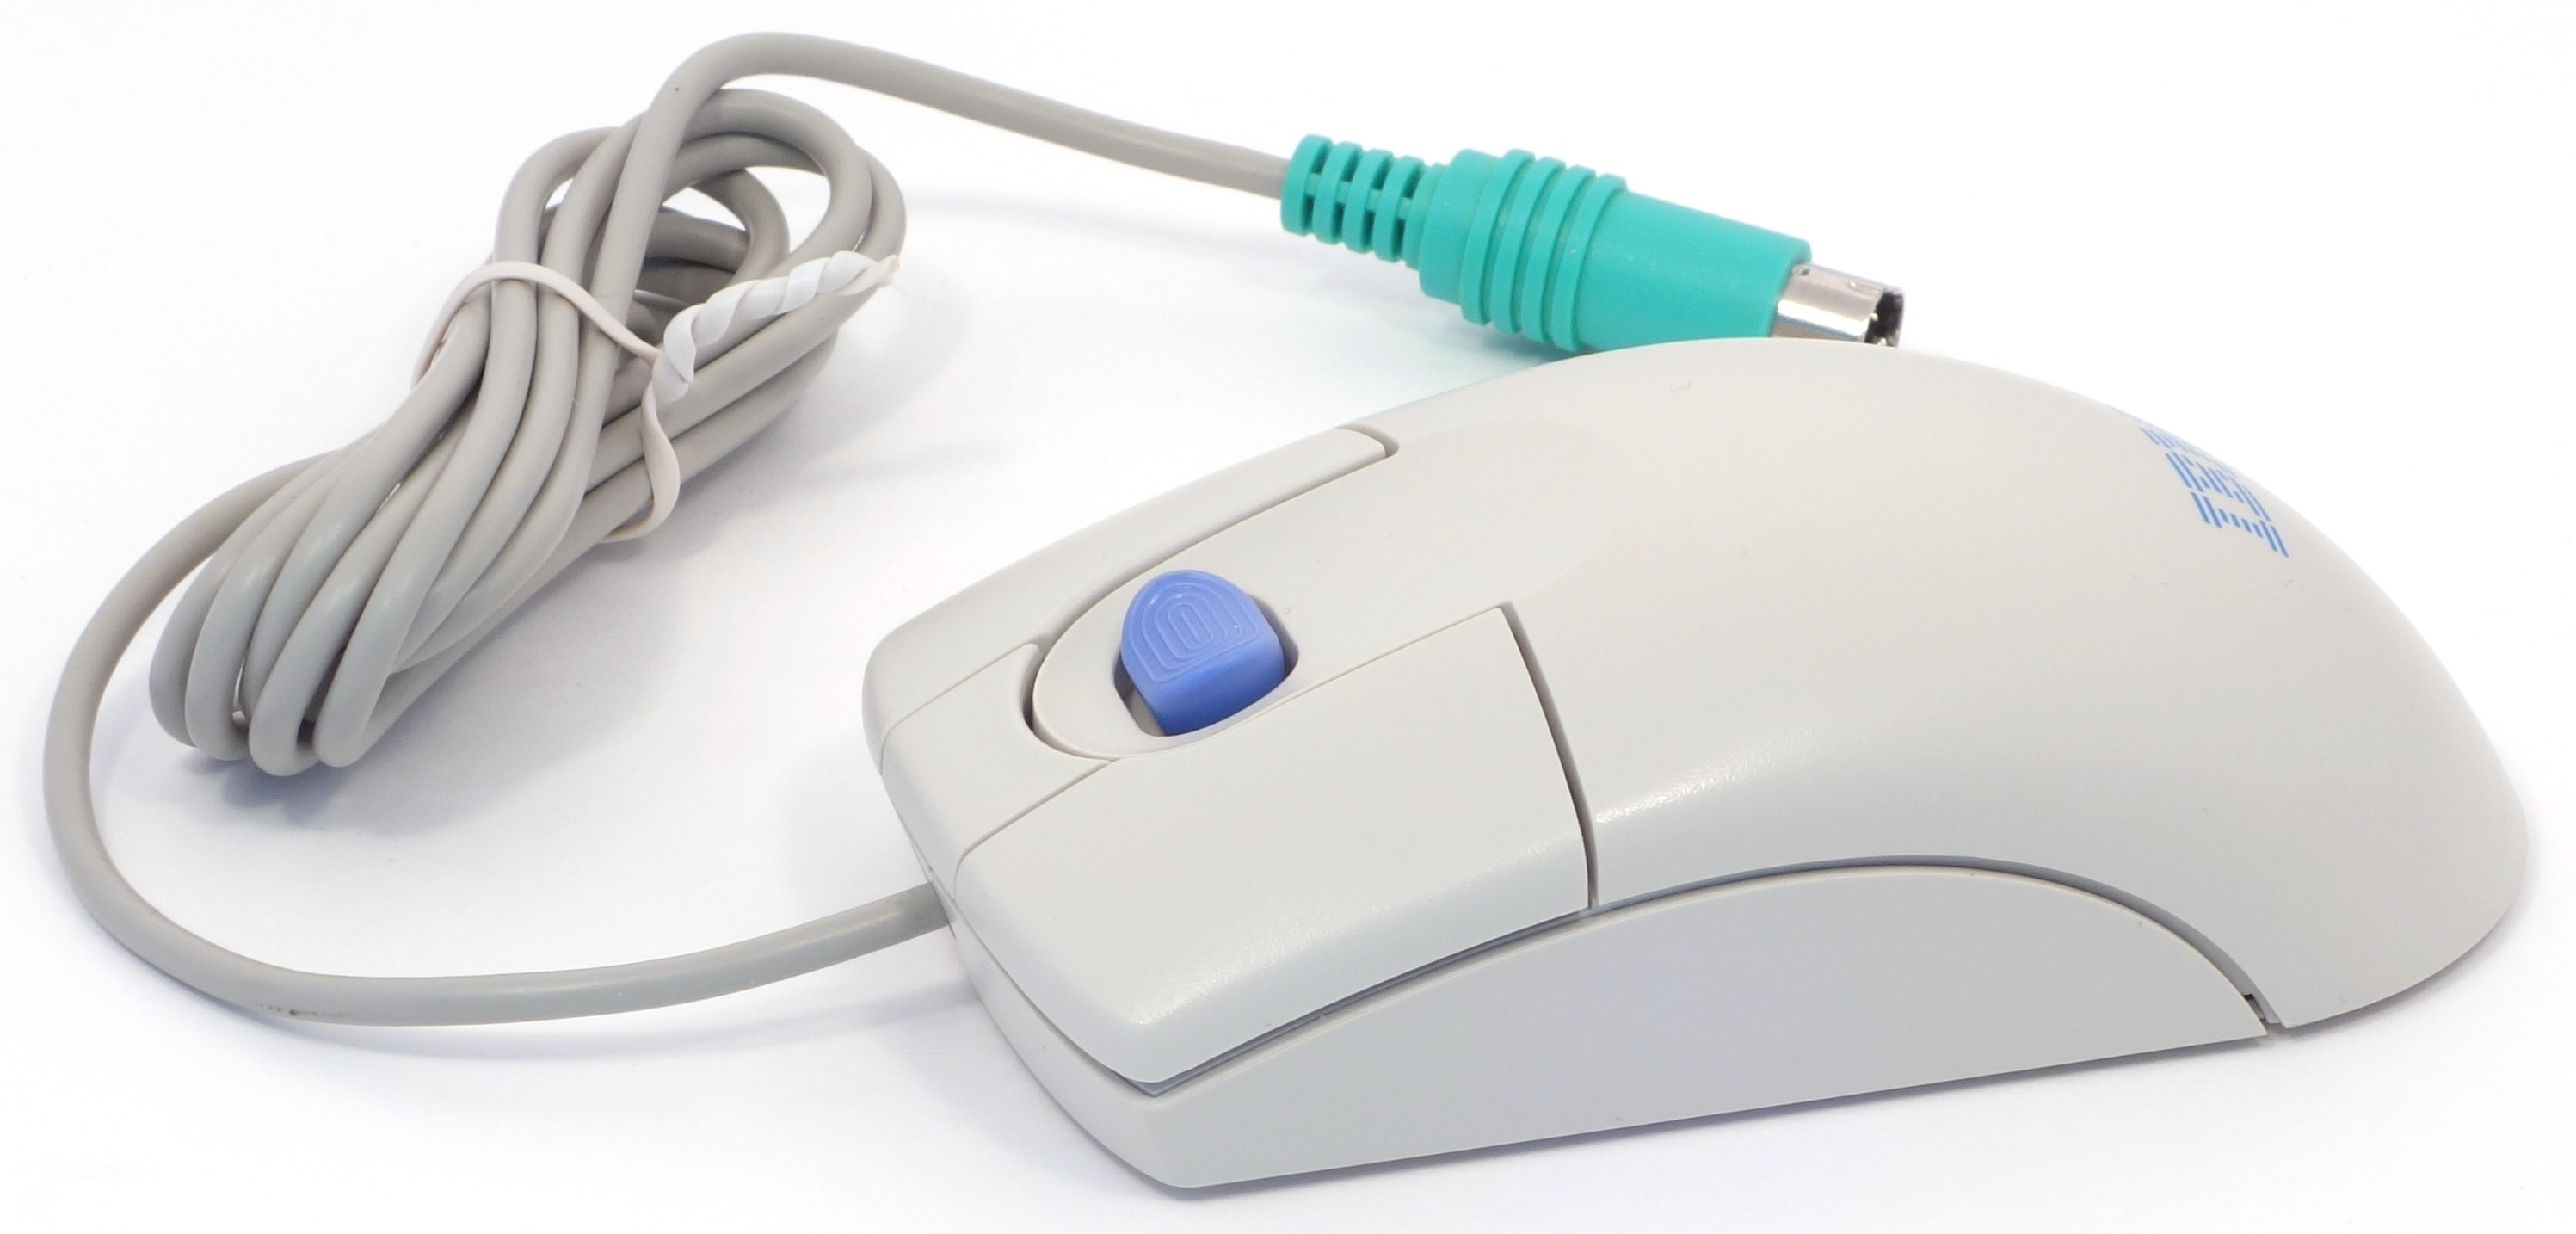
\includegraphics[scale=0.6]{2000_ibm_scrollpoint_ii_mouse/pic_30.jpg}
    \caption{IBM ScrollPoint II mouse}
    \label{fig:IBMScrollPointIIPic}
\end{figure}

Второе поколение мыши ScrollPoint получило корпус чуть более округлой формы, новую форму резинового наконечника джойстика, а также третью кнопку, расположенную непосредственно за ним (рис. \ref{fig:IBMScrollPointIITopBottom}).

\begin{figure}[h]
    \centering
    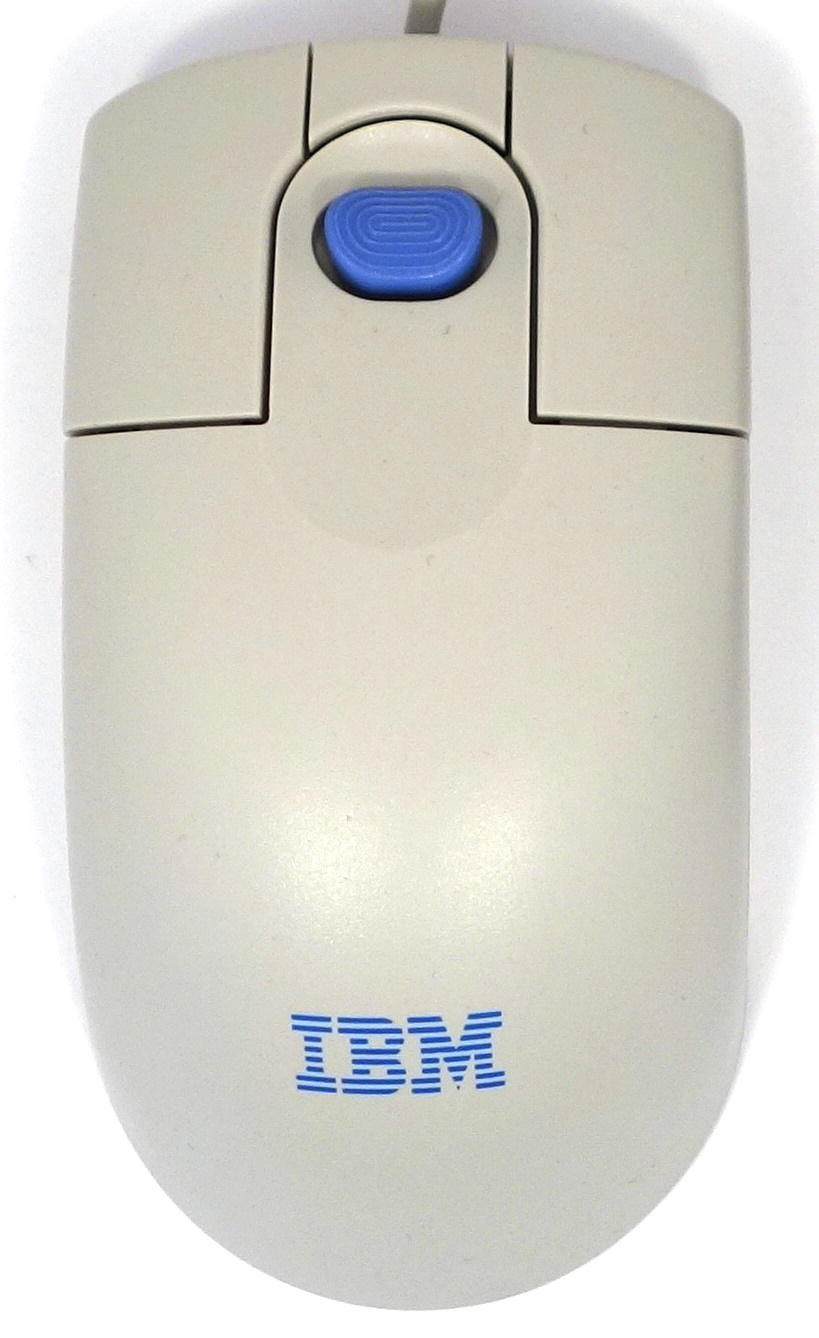
\includegraphics[scale=0.7]{2000_ibm_scrollpoint_ii_mouse/top_30.jpg}
    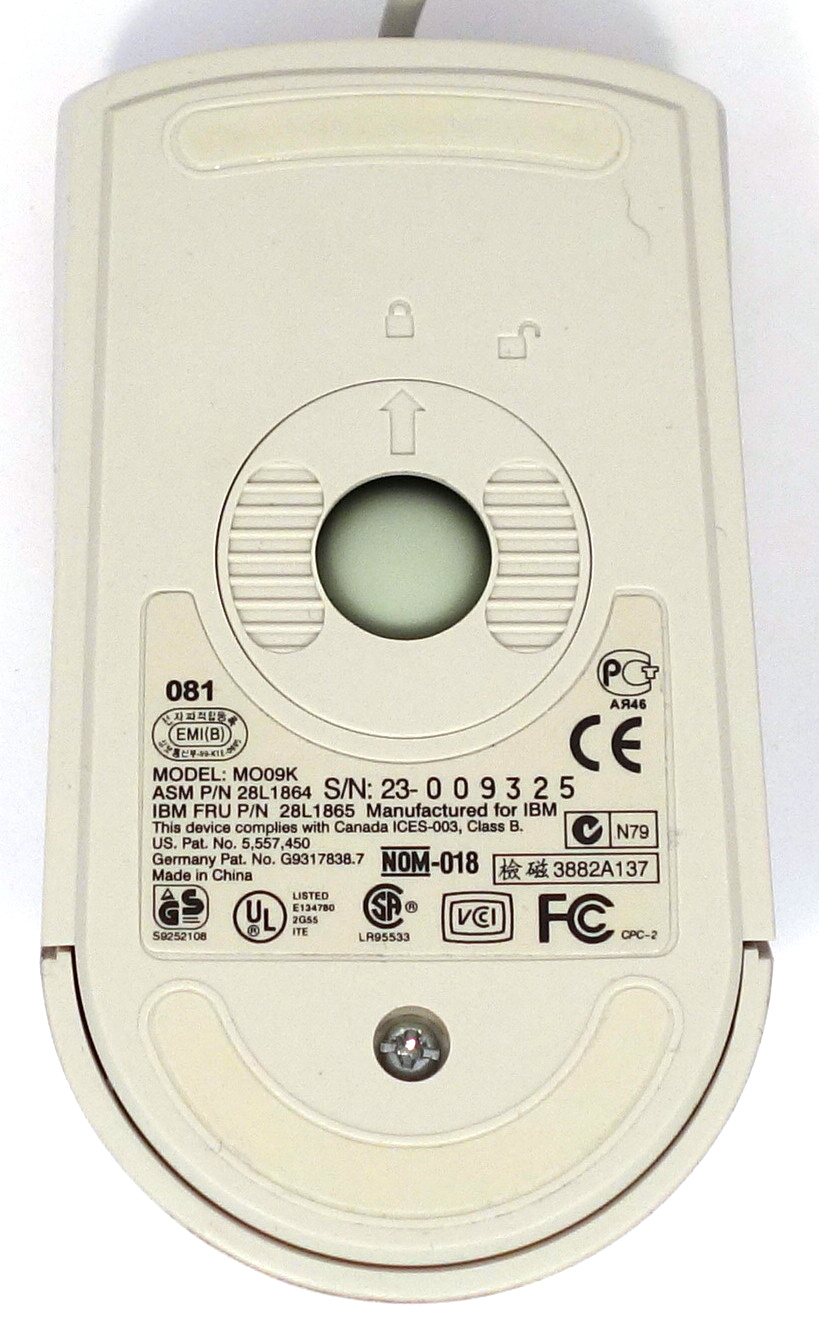
\includegraphics[scale=0.7]{2000_ibm_scrollpoint_ii_mouse/bottom_30.jpg}
    \caption{IBM ScrollPoint II mouse, вид сверху и снизу}
    \label{fig:IBMScrollPointIITopBottom}
\end{figure}

Замена традиционного для ноутбуков круглого наконечника трекпоинта на подобие вогнутой ребристой качельки было призвано облегчить горизонтальный скроллинг. Как известно, пальцы приспособлены к приложению усилия вбок меньше, чем вниз. По замыслу разработчиков, вертикальное нажатие средним пальцем вблизи от края вогнутой поверхности должно за счет эффекта рычага облегчать горизонтальную прокрутку \cite{buxtonG2}.

\begin{figure}[h]
    \centering
    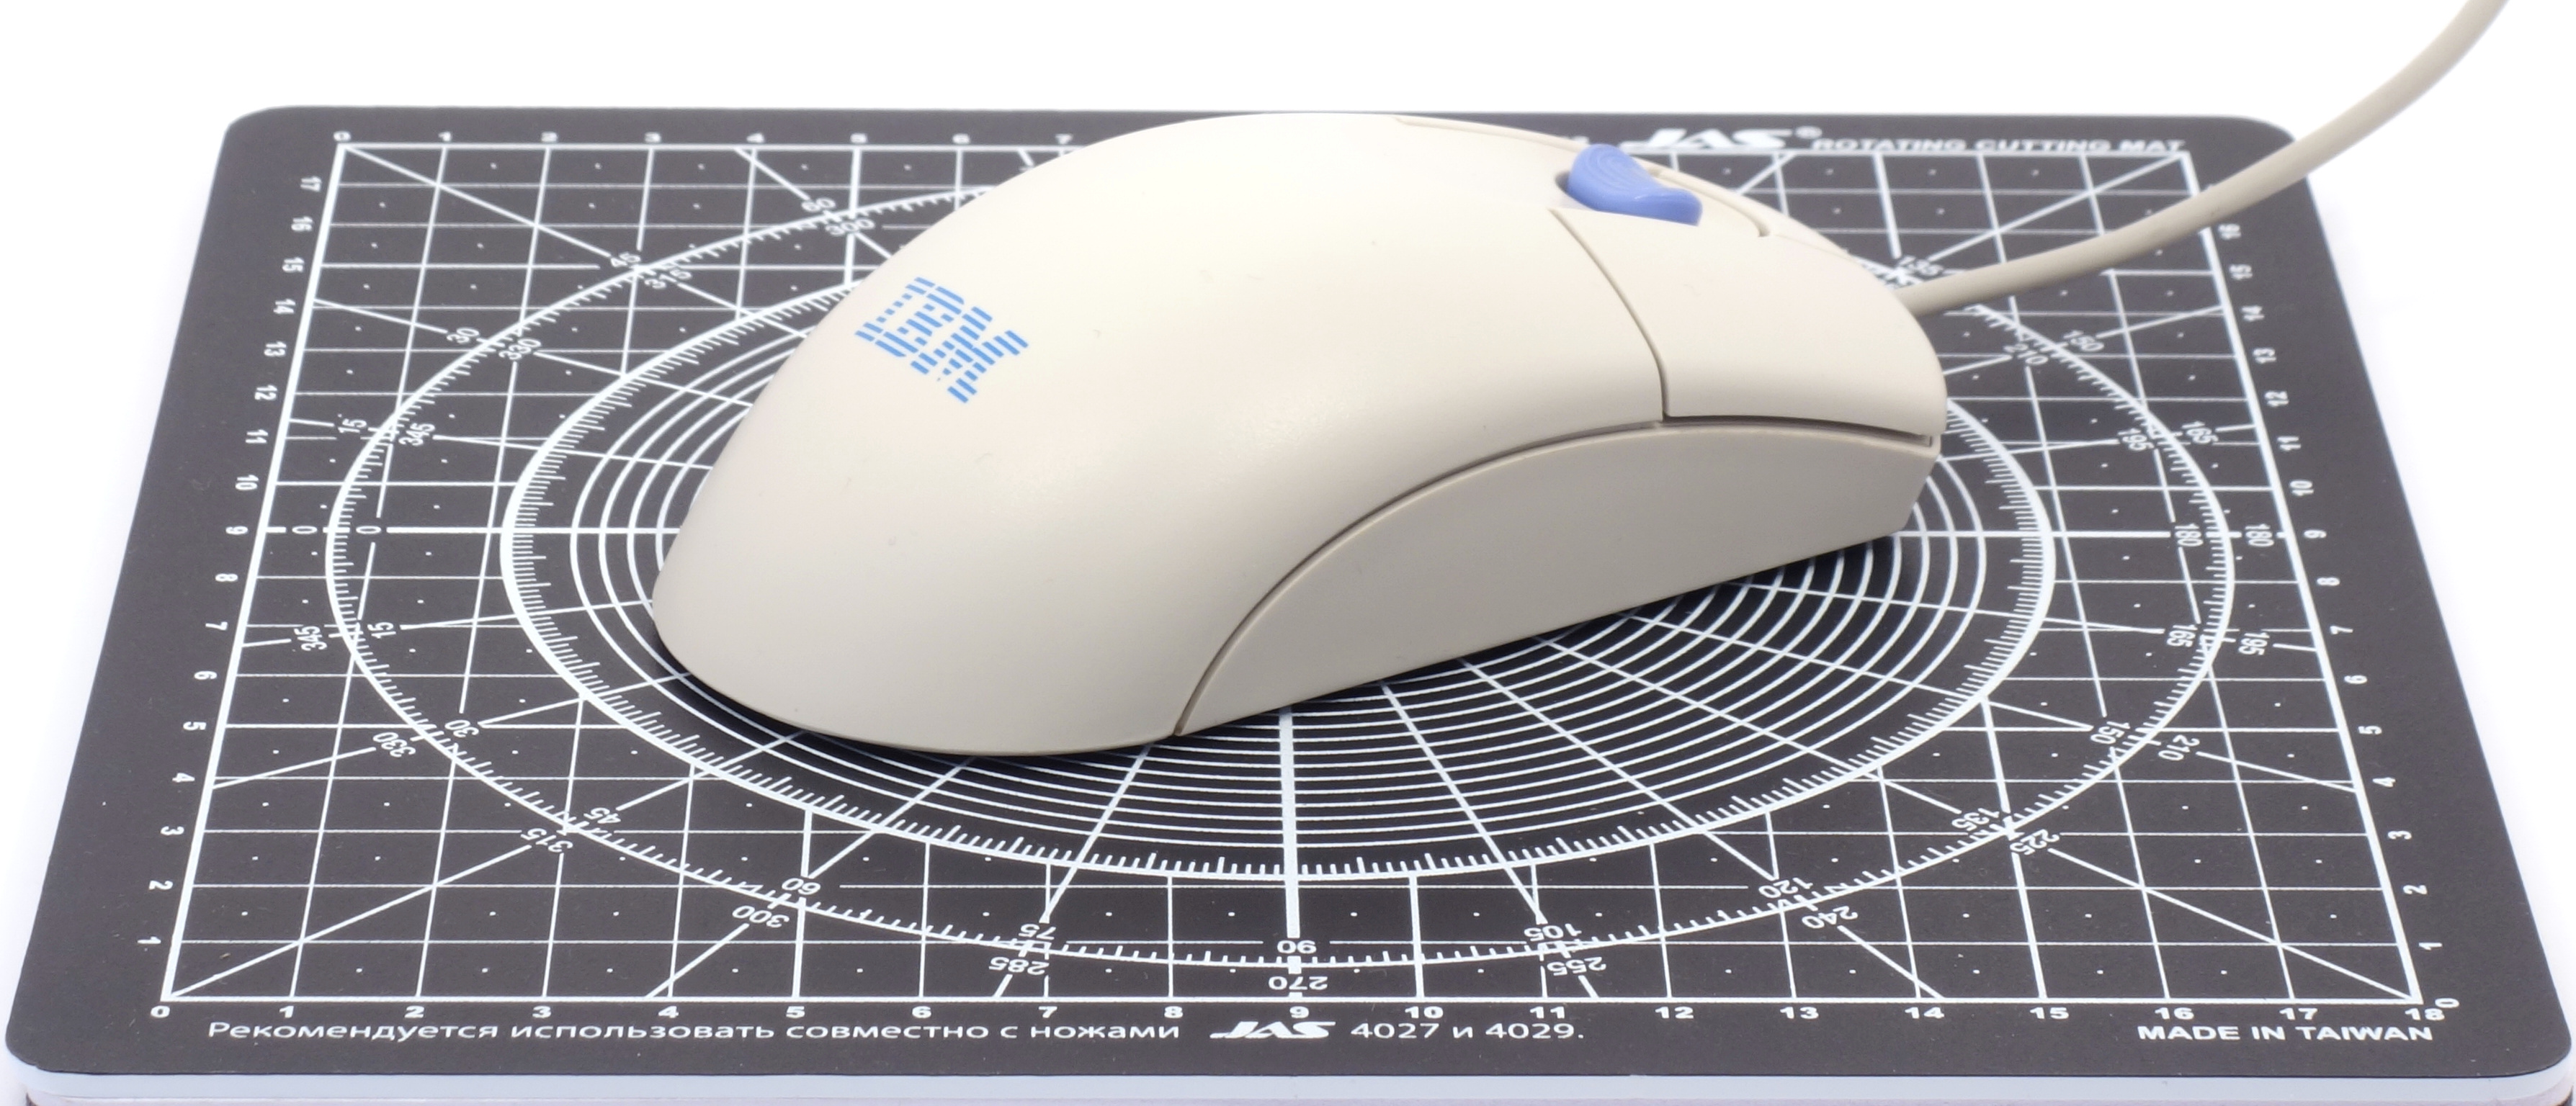
\includegraphics[scale=0.54]{2000_ibm_scrollpoint_ii_mouse/size_30.jpg}
    \caption{Изображение IBM ScrollPoint II mouse на размерном коврике с шагом сетки 1~см}
    \label{fig:IBMPS2Size}
\end{figure}

Как можно видеть на рис. (рис. \ref{fig:IBMPS2Size}), мышь имеет типичные средние размеры. Изогнутая форма корпуса позволяет комфортно опереться на неё ладонью  \ref{fig:IBMScrollPointIIHand} и нажимать кнопки при естественном положении кисти. При этом корпус симметричен и одинаково подходит для левшей и правшей.


\begin{figure}[h]
    \centering
    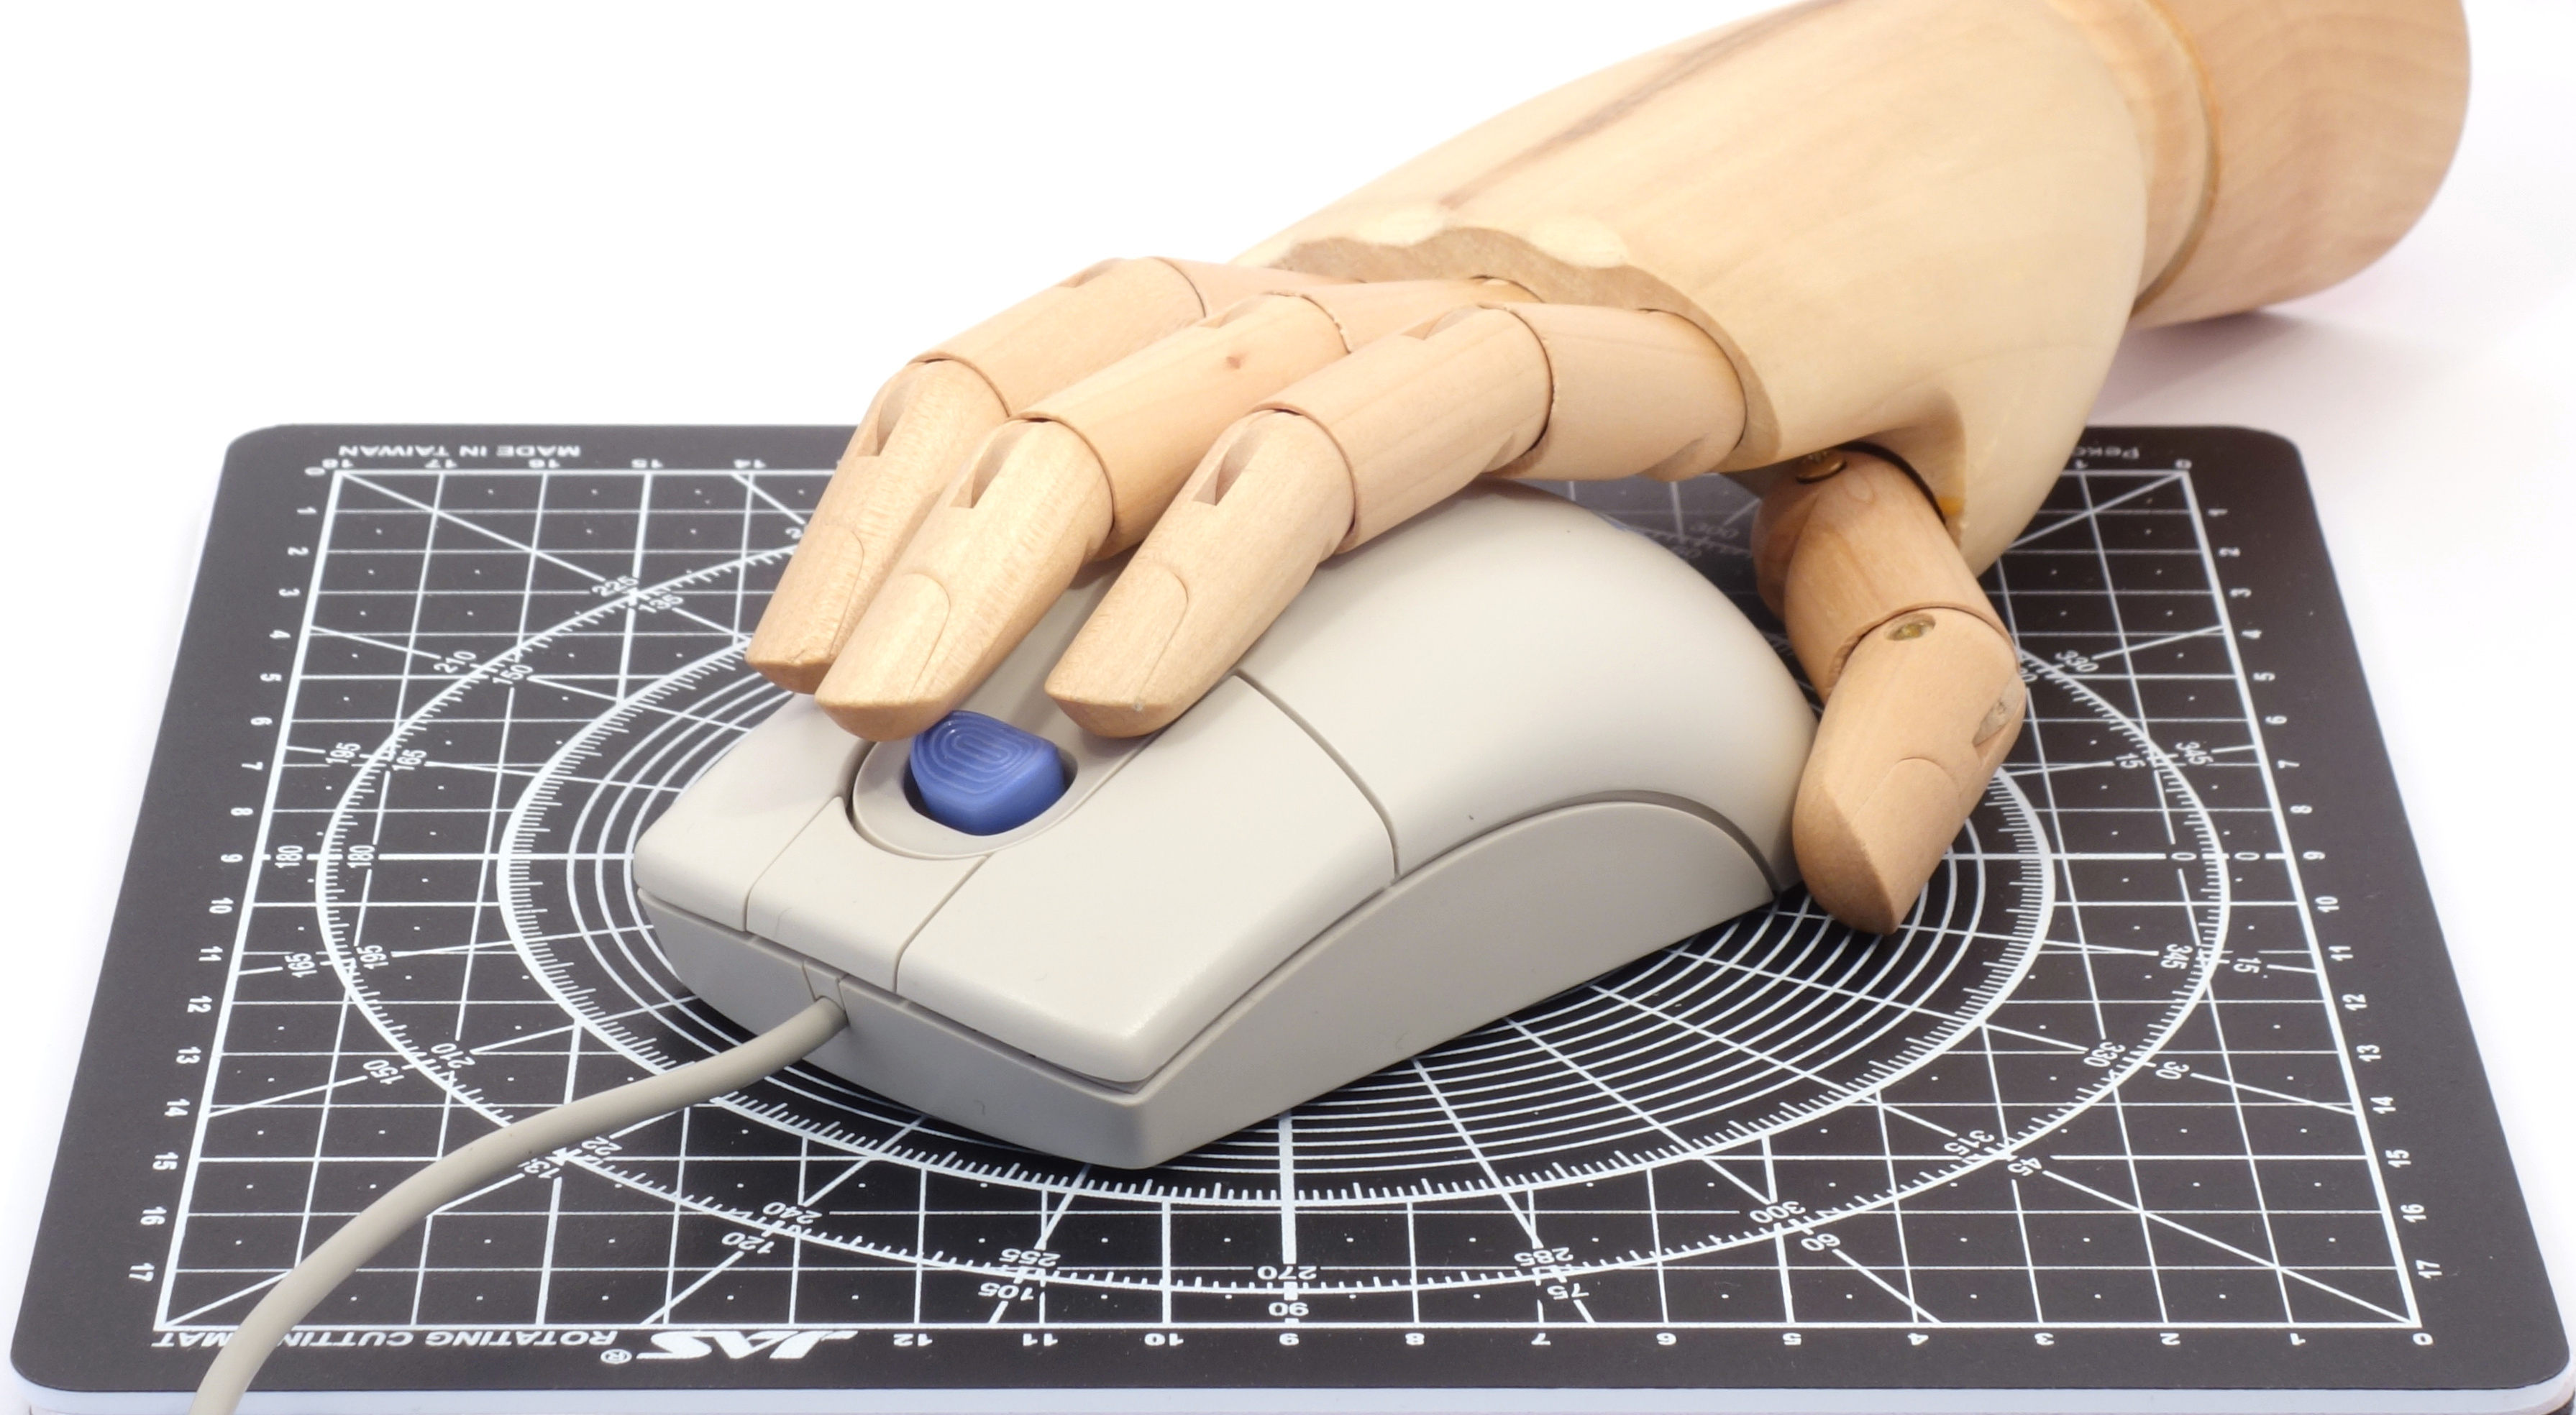
\includegraphics[scale=0.6]{2000_ibm_scrollpoint_ii_mouse/hand_30.jpg}
    \caption{Изображение IBM ScrollPoint II mouse с моделью руки человека}
    \label{fig:IBMScrollPointIIHand}
\end{figure}

Внутреннее устройство IBM ScrollPoint II mouse показано на рис. \ref{fig:IBMPS2Inside}, что позволяет классифицировать мышь как типовое (помимо наличия тензометрического джойстика) устройство с оптомеханическим энкодером. Однако конструкция мыши демонстрирует отчетливые признаки консерватизма: характерным примером является защита шара, типичная для первой половины девяностых годов, но не слишком характерная для для манипуляторов 2000 года выпуска.

\begin{figure}[h]
    \centering
    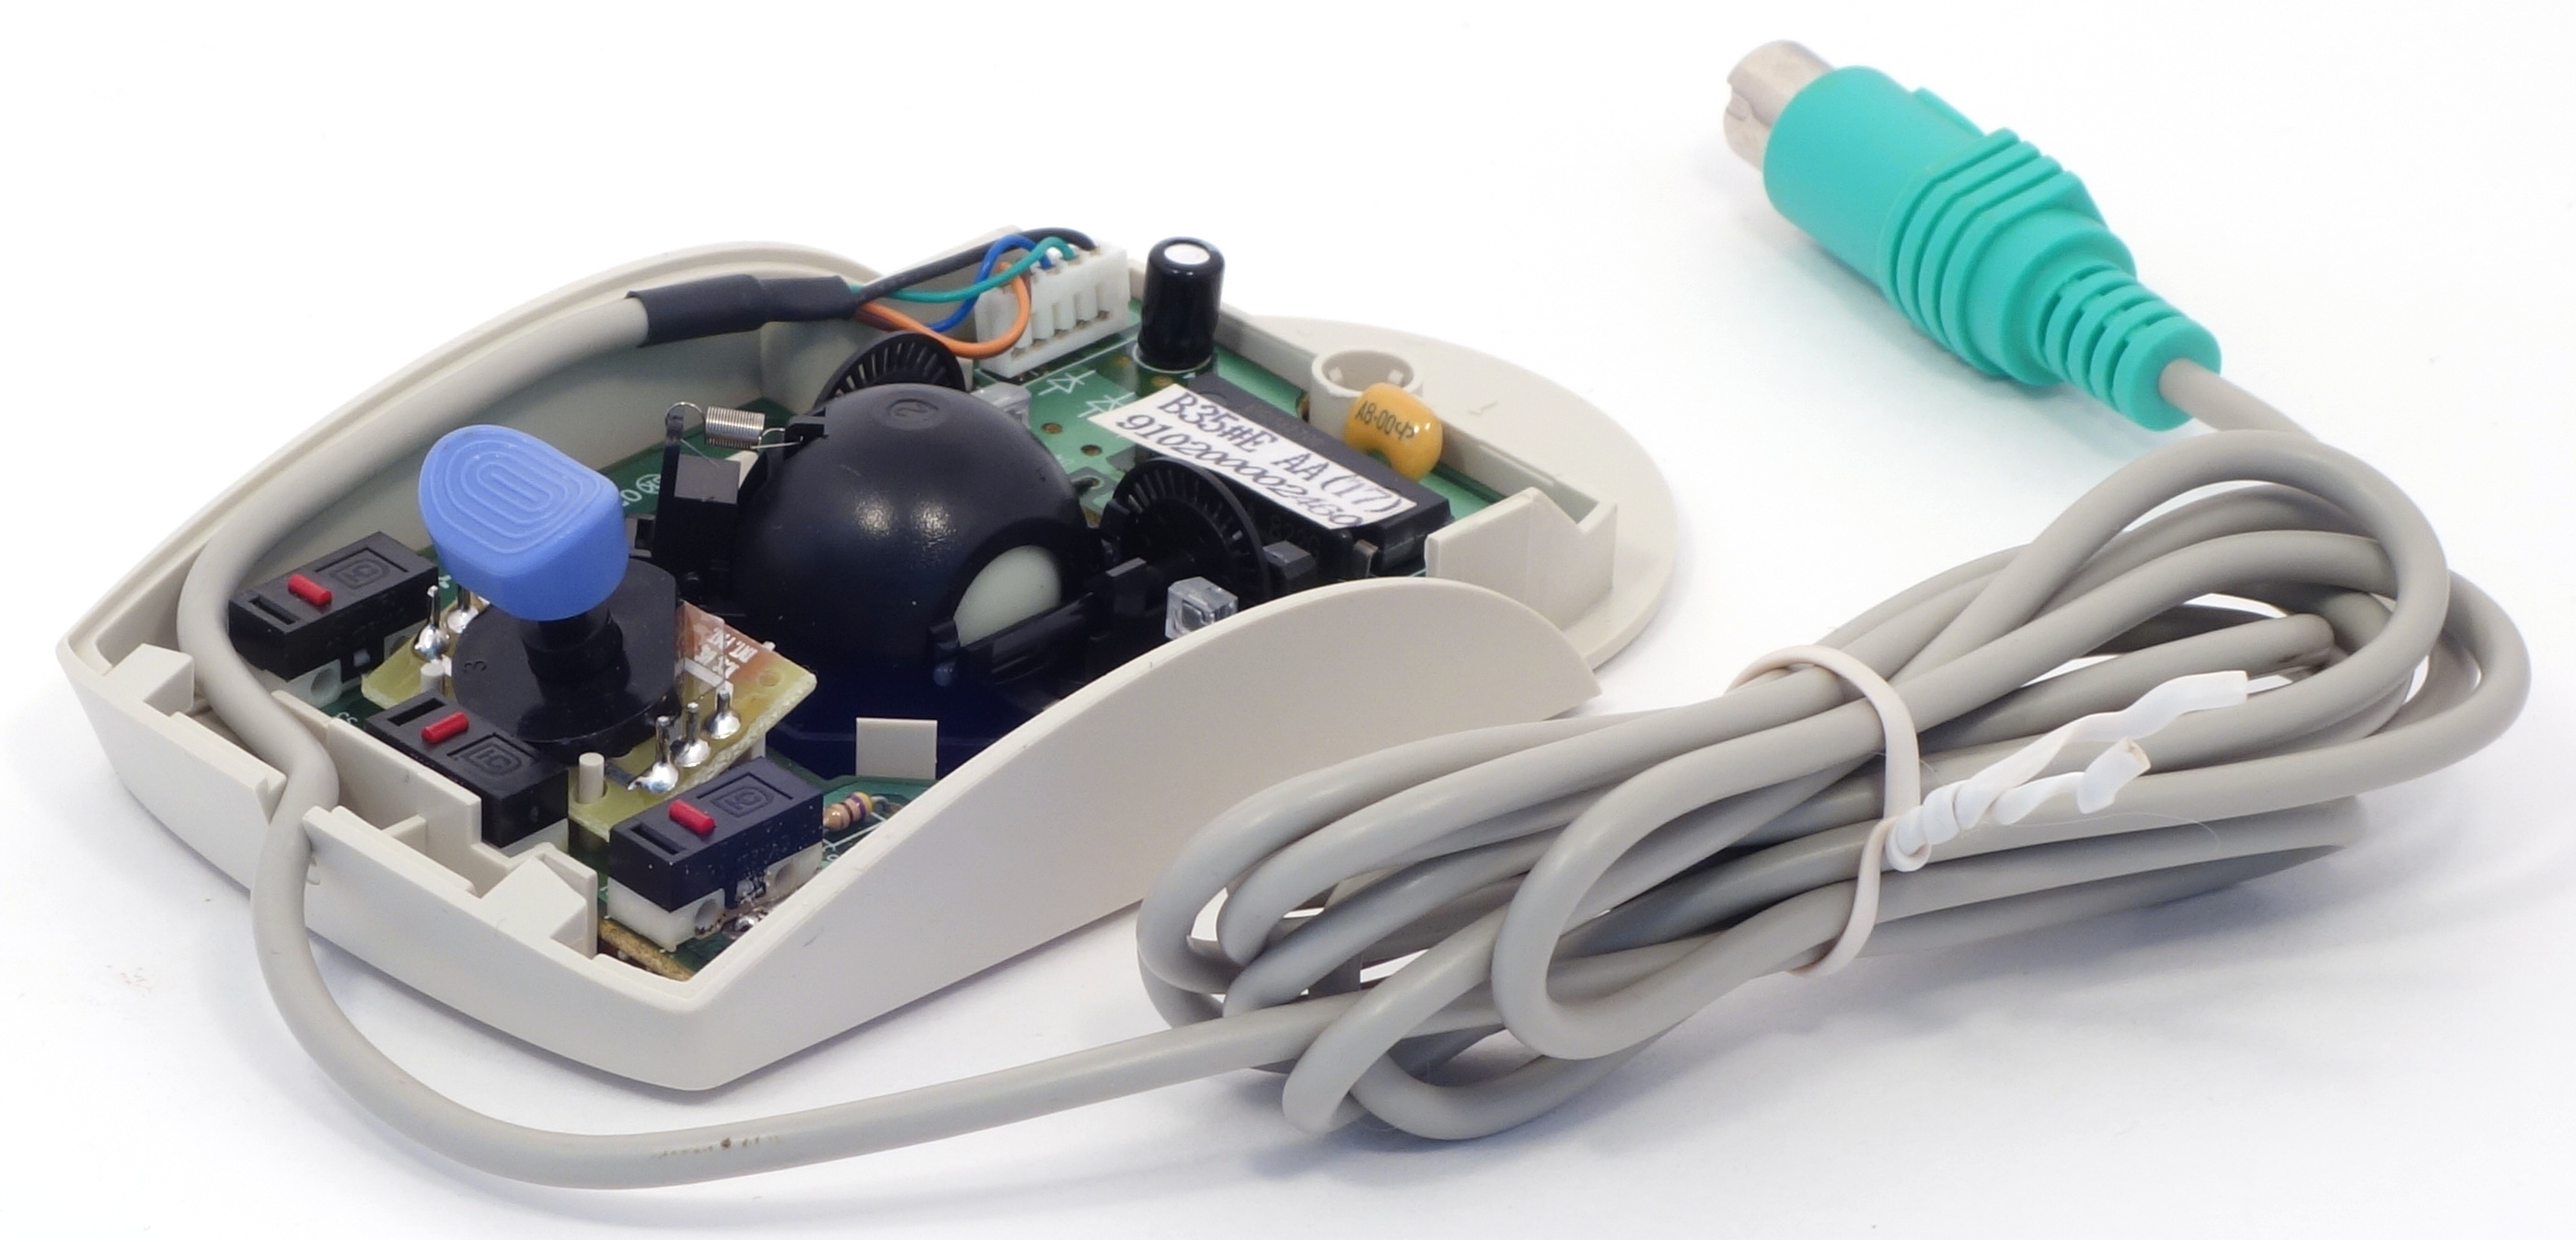
\includegraphics[scale=0.7]{2000_ibm_scrollpoint_ii_mouse/inside_30.jpg} 
    \caption{IBM ScrollPoint II mouse в разобранном состоянии}
    \label{fig:IBMPS2Inside}
\end{figure}

\begin{thebibliography}{9}
    \bibitem {buxtonG1} Bill Buxton. TrackPoint Mouse G1 -- Buxton Collection. \url{https://www.microsoft.com/buxtoncollection/detail.aspx?id=120}
    \bibitem {buxtonG2} Bill Buxton. TrackPoint Mouse G2 -- Buxton Collection. \url{https://www.microsoft.com/buxtoncollection/detail.aspx?id=121}
    \bibitem {hist} IBM ScrollPoint Information and Software -- ibmfiles.com // \url{http://www.ibmfiles.com/pages/scrollpoint.htm}
\end{thebibliography}

\end{document}
